\documentclass[../PS6_RapportFinal.tex]{subfiles}

\begin{document}
\graphicspath{{img/}{tex/img/}}
\subsection{Chaleur dégagée par la réaction de décomposition  }
 
Pour pouvoir comparer le pouvoir calorifique du compost avec celui d’autres combustibles, il faut calculer la chaleur dégagée par le bois lors de sa décomposition. Ainsi on pourra savoir si le chauffage à l'aide du compost est viable.

On rappelle la réaction :

\[C_aH_bO_cN_d + \frac{4a + b - 2c -3d}{4}O_2 \longrightarrow aCO_2+ \frac{b-3d}{2} H_2O + dNH_3\]

\textbf{Hypothèses :}
\begin{itemize}
\item On considère la réaction comme totale 
\item Le bois est composé de 73\% de cellulose et de 27\% de lignine %References

\item La réaction se déroule à une température de 298 \si{\kelvin} (25 \si{\degreeCelsius})
\item La réaction se déroule à la pression atmosphérique 
\end{itemize}
 
Pour calculer l’énergie maximale dégagée par la réaction on va utiliser la loi de Hess qui dit que l'enthalpie standard de la réaction est égale à la somme des énergies de liaison de toutes les molécules présentes dans la réaction:

\[\Delta_r H^o(T) = \sum_i \nu_i \Delta_{f,i}H^o(T) \text{ avec }\nu_i < 0 \text{ pour les réactifs et }>0 \text{ pour les produits}\] 

Tout d’abord il est nécessaire de rappeler les formules brutes des composants du bois et des autres molécules intervenant dans la réaction :
\begin{description}
\item La cellulose : \(C_6 H_{10} O_5\) %\chemfig{C([3]=O)([5]-H)-C([2]-H)([6]-O-H)-C([2]-O-H)([6]-H)-C([2]-H)([6]-O-H)-C([2]-O-H)([6]-H)-C([9]=O)([7]-H)}
\item La lignine : polymère de monomères \(C_9 H_{10} O_2\) ou \(C_{10} H_{12} O_3\) ou \(C_{11} H_{14} O_4\)

\item Le dioxygène : \(O_2\) \
%\chemfig{O=O}
\item Le dioxyde de carbone : \(CO_2\)
%\chemfig{O=[:30]C=[:30]O}
\item L'eau : \(H_2O\)
%\chemfig{H-[:30]O-[:30]H}
\end{description}

\vspace{3mm}

Pour la cellulose et les monomères de la lignine, il faut savoir que ce sont des composés cycliques.

Il est aussi indispensable de connaître les énergies des liaisons présentes dans les molécules réagissant (\fref{tab-NRJ_liaison}) ainsi que la masse molaire des différents composés du bois (\fref{tab-MassesMolBois}).

\begin{table}[!h]
\begin{center}
\begin{tabular}{|c|c|c|}
\hline
Liaison chimique & \(\Delta_r H^{o}\) & Notations (à 298 \si{\kelvin}) [\si{\kilo\joule\per\mole}] \\ \hline
\chemfig{O-H} & 464 & \(\Delta_{OH'} H^{o}\) \\ \hline
\chemfig{O-C} & 351 & \(\Delta_{CO'} H^{o}\) \\ \hline
\chemfig{C-H} & 414 & \(\Delta_{CH'} H^{o}\) \\ \hline
\chemfig{O=O} & 502 & \(\Delta_{OO''} H^{o}\) \\ \hline
%\chemfig{C=C} & 615 & \(\Delta_{CC''} H^{o}\) \\ \hline
\chemfig{C=O} & 730 & \(\Delta_{CO''} H^{o}\) \\ \hline
\chemfig{C-C} & 347 & \(\Delta_{CC'} H^{o}\) \\ \hline
\end{tabular}
\caption{Énergies de liaison utiles et notations}
\label{tab-NRJ_liaison}
\end{center}
\end{table}

\begin{table}[!h]
\begin{center}
\begin{tabular}{|c|c|}
\hline
Composé & Masse molaire [\si{\kilo\joule\per\mole}] \\ \hline
Cellulose & 162 \\ \hline
Lignine & 150 \\ \hline
\end{tabular}
\caption{Masses molaires des composés du bois}
\label{tab-MassesMolBois}
\end{center}
\end{table}

\subsubsection{Dégradation de la cellulose}

L'équation chimique de la décomposition de la cellulose est la suivante :
\[C_6H_{10}O_5 + 6O_2 \longrightarrow 6CO_2 + 5H_2O\]

D'après la loi de Hess :
\begin{multline*}
\Delta_{cellulose}H^o = 10 \Delta_{\tiny CO''} H^o  + 7 \Delta_{\tiny OH'} H^o - 6 \Delta_{\tiny OO''} H^o - 5 \Delta_{\tiny CC'} H^o  - 3 \Delta_{\tiny CO'} H^o  - 7 \Delta_{\tiny CH'} H^o
\end{multline*}
\[ \Rightarrow\Delta_{cellulose} H^o (298 \: \si{\kelvin}) = 1850 \: \si{\kilo\joule\per\mole}\]

\subsubsection{Dégradation de la lignine}
L'équation chimique de la décomposition de la lignine est la suivante :
\[2C_9H_{10}O_2 + 21O_2 \longrightarrow 18CO_2 + 10H_2O\]

D'après la loi de Hess :
\begin{multline*}
\Delta_{lignine} H^o  = 34 \Delta_{\tiny CO''} H^o + 20 \Delta_{\tiny OH'} H^o - 21 \Delta_{\tiny OO''} H^o - 8 \Delta_{\tiny CC'} H^o  - 8\Delta_{\tiny CC''} H^o  - 16\Delta_{\tiny CH'} H^o 
\end{multline*}
\[ \Rightarrow\Delta_{lignine} H^o (298 \: \si{\kelvin}) = 9238 \: \si{\kilo\joule\per\mole} \]

On remarque que la dégradation de la lignine produit plus de chaleur que la dégradation de la cellulose. Ainsi pour avoir un maximum de chaleur il faudrait utiliser un bois qui est composé d'un maximum de lignine.

\subsubsection{Conclusion}

Le bois étant composé de lignine et de cellulose on peut ainsi calculer le pouvoir calorifique du bois. 
\[\Delta_{bois} H^o (298 \: \si{\kelvin}) =\num{0.73} \Delta_{cellulose} H^o (298  \: \si{\kelvin})+ \num{0.27}\Delta_{lignine} H^o (298  \: \si{\kelvin}) = \num{4066.4} \: \si{\kilo\joule\per\mole}\]  
soit \(\Delta_{bois} H^o (298 \: \si{\kelvin}) = \num{25.6} \: \si{\kilo\joule\per\kilogram}\)

Si on compare le pouvoir calorifique (énergie récupérable par unité de masse) de la décomposition du bois avec celui d’autres combustibles usuels on note que le compost peut être une énergie viable (\fref{fig-ComparaisonNRJ}).

\begin{figure}[!h]
\begin{center}
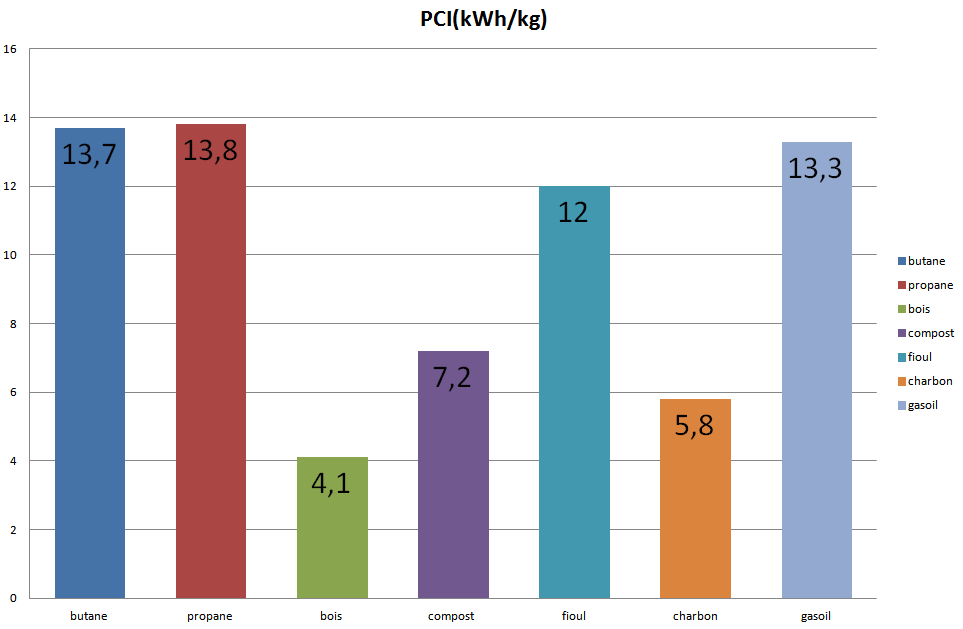
\includegraphics[scale=0.5]{1_2_Graphique_comparaison_energie.png}
\caption{Comparaison du pouvoir calorifique de différentes combustibles}
\label{fig-ComparaisonNRJ}
\end{center}
\end{figure}

On observe que le compost peut être intéressant car son pouvoir calorifique est supérieur à celui du bois de chauffage.Cependant, ce pouvoir calculé suppose que la réaction soit totale or ce n’est pas le cas. Néanmoins, on peut tendre vers cette valeur si on humidifie le tas de compost régulièrement et si on amène de l’oxygène en excès.

\end{document}